\documentclass[12pt, twoside]{article}
\input{/Users/chris/github/course-files/docs/ib/preamble}

\fancyhead[LE]{\thepage}
\fancyhead[RO]{Markscheme}
\fancyhead[LO]{La Scuola d'Italia / Dr.\ Huson / IB Math 12 HL \\* 30 September 2026}

\begin{document}
\subsubsection*{5.2 Classwork: Calculus Review (no calculator) --- Markscheme}

\emph{Total: 38 marks. All four problems are past IB AA HL questions; the
mark allocations follow the official markschemes.}

\begin{enumerate}[itemsep=0.3cm]

%--- Problem 1: sec x Maclaurin series from cos x and (1+t)^-1; limit with arctan 2x [8 marks] ---
%--- Source: AA HL 2021 May P2 TZ2 Q09 ---
\item[1.] \makebox[\linewidth][s]{[Maximum mark: 8]\hfill {\small AA HL 2021 May P2 TZ2 Q9}}

\textbf{(a)} $(1 + t)^{-1} = 1 - t + t^{2}$ \hfill \textbf{A1}

\emph{Accept the three terms listed: $1$, $-t$, $t^{2}$.}

\medskip

\textbf{(b)} $\sec x = \dfrac{1}{\cos x}
= \dfrac{1}{1 - \frac{x^{2}}{2!} + \frac{x^{4}}{4!} - \cdots}$
\hfill \textbf{(M1)}

Let $t = \cos x - 1 = -\dfrac{x^{2}}{2} + \dfrac{x^{4}}{24} - \cdots$, so
$\sec x = 1 - t + t^{2}$ \hfill \textbf{(M1)}

$= 1 - \left(-\dfrac{x^{2}}{2} + \dfrac{x^{4}}{24}\right)
+ \left(-\dfrac{x^{2}}{2} + \dfrac{x^{4}}{24}\right)^{2} + \cdots$
\hfill \textbf{A1}

$= 1 + \dfrac{x^{2}}{2} - \dfrac{x^{4}}{24} + \dfrac{x^{4}}{4} + \cdots$
\hfill \textbf{A1}

$= 1 + \dfrac{x^{2}}{2} + \dfrac{5x^{4}}{24}$ \hfill \textbf{AG}

\emph{The second A1 needs both $x^{4}$ contributions, $-\dfrac{x^{4}}{24}$
and $+\dfrac{x^{4}}{4}$ (from squaring $-\dfrac{x^{2}}{2}$), seen before the
given answer. Condone the absence of ``$\cdots$''.}

\emph{Differentiating $\sec x$ four times earns no marks: the question
requires the method of parts (a) and (b).}

\medskip

\textbf{(c)} $\arctan 2x = 2x - \dfrac{(2x)^{3}}{3} + \cdots$

$\displaystyle\lim_{x \to 0}\frac{x\left(2x - \frac{8x^{3}}{3} + \cdots\right)}
{\left(1 + \frac{x^{2}}{2} + \frac{5x^{4}}{24}\right) - 1}$
\hfill \textbf{M1}

$\displaystyle = \lim_{x \to 0}\frac{2x^{2} - \frac{8x^{4}}{3} + \cdots}
{\frac{x^{2}}{2} + \frac{5x^{4}}{24}}
= \lim_{x \to 0}\frac{2 - \frac{8x^{2}}{3} + \cdots}{\frac{1}{2} + \frac{5x^{2}}{24}}$
\hfill \textbf{A1}

$= 4$ \hfill \textbf{A1}

\emph{Do not award the M1 unless $x$ is replaced by $2x$ in the
$\arctan$ series. Condone a missing ``$\lim$'' and errors in the
higher-order terms. Only the leading terms $2x^{2}$ and $\dfrac{x^{2}}{2}$
are needed for the answer.}

\emph{L'H\^opital's rule gives the same limit but earns no marks: the
question requires the Maclaurin series.}

\newpage

%--- Problem 2: kinematics, v = 4 + 4t - 3t^2 [16 marks] ---
%--- Source: AA HL 2021 Nov P1 TZ0 Q10 ---
\item[2.] \makebox[\linewidth][s]{[Maximum mark: 16]\hfill {\small AA HL 2021 Nov P1 Q10}}

$v(t) = 4 + 4t - 3t^{2}$, \ $0 \leq t \leq 3$; \ $P$ at $O$ when $t = 0$.

\medskip

\textbf{(a)(i)} Valid approach to find the turning point:
$v'(t) = 4 - 6t = 0$ \hfill \textbf{(M1)}

$t = \dfrac{2}{3}$ (s) \hfill \textbf{A1}

\emph{Accept $t = -\dfrac{b}{2a} = -\dfrac{4}{2(-3)}$, or the average of the
roots $\dfrac{-\frac{2}{3} + 2}{2}$.}

\textbf{(a)(ii)} Attempt to integrate $v$ \hfill \textbf{(M1)}

$\displaystyle\int (4 + 4t - 3t^{2})\, dt = 4t + 2t^{2} - t^{3} \ (+c)$
\hfill \textbf{A1A1}

\emph{A1 for $4t + 2t^{2}$, A1 for $-t^{3}$.}

Since $s(0) = 0$, $c = 0$. Substitute $t = \dfrac{2}{3}$: \hfill \textbf{(M1)}

$4\left(\dfrac{2}{3}\right) + 2\left(\dfrac{2}{3}\right)^{2}
- \left(\dfrac{2}{3}\right)^{3}
= \dfrac{8}{3} + \dfrac{8}{9} - \dfrac{8}{27}$ \hfill \textbf{A1}

$= \dfrac{72 + 24 - 8}{27} = \dfrac{88}{27}$ (m) \hfill \textbf{AG}

\emph{The A1 needs the three fractions (or an equivalent line) before the
given answer.}

\medskip

\textbf{(b)} Solve $4 + 4t - 3t^{2} = 0$: $(2 - t)(2 + 3t) = 0$
\hfill \textbf{(M1)}

\begin{center}
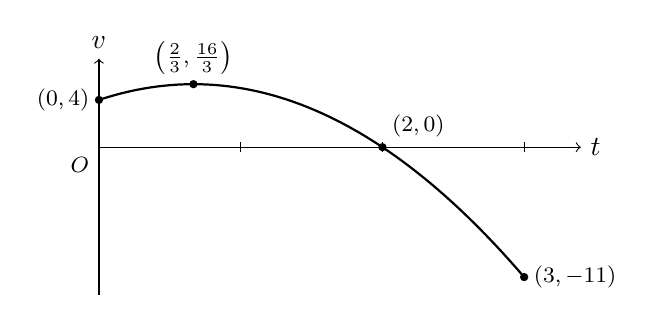
\begin{tikzpicture}[x=1.8cm, y=0.15cm]
  \draw[->] (0,0) -- (3.4,0) node[right] {$t$};
  \draw[->] (0,-12.5) -- (0,7.5) node[above] {$v$};
  \foreach \t in {1,2,3} \draw (\t,0.4)--(\t,-0.4);
  \node[below left] at (0,0) {\footnotesize $O$};
  \draw[thick, domain=0:3, samples=60] plot (\x, {4 + 4*\x - 3*\x*\x});
  \fill (0,4) circle (1.5pt) node[left] {\footnotesize $(0, 4)$};
  \fill (2,0) circle (1.5pt) node[above right] {\footnotesize $(2, 0)$};
  \fill (2/3,16/3) circle (1.5pt) node[above] {\footnotesize $\left(\frac{2}{3}, \frac{16}{3}\right)$};
  \fill (3,-11) circle (1.5pt) node[right] {\footnotesize $(3, -11)$};
\end{tikzpicture}
\end{center}

Correct $t$-intercept at $t = 2$ \hfill \textbf{A1}

Correct domain from $0$ to $3$, starting at $(0, 4)$ \hfill \textbf{A1}

Vertex in approximately the correct place: $t = \dfrac{2}{3}$, $v > 4$
\hfill \textbf{A1}

\emph{The last two A marks are awarded only if the shape is a concave-down
parabola; they are independent of each other and of the (M1). The end at
$t = 3$ must be clearly shown; the value $v(3) = -11$ need not be labelled.
The root $t = -\dfrac{2}{3}$ is outside the domain and must not be drawn.}

\medskip

\textbf{(c)} Integrate over $[0, 2]$ and $[2, 3]$ ($P$ turns at $t = 2$)
\hfill \textbf{(M1)}

$\displaystyle\int_{0}^{2}(4 + 4t - 3t^{2})\, dt = 8$ \hfill \textbf{A1}

$\displaystyle\int_{2}^{3}(4 + 4t - 3t^{2})\, dt = 3 - 8 = -5$
\hfill \textbf{A1}

Valid approach to sum the two distances:
$\displaystyle\int_{0}^{2} v\, dt - \int_{2}^{3} v\, dt$ \hfill \textbf{(M1)}

Total distance travelled $= 8 + 5 = 13$ (m) \hfill \textbf{A1}

\emph{$\displaystyle\int_{0}^{3} v\, dt = 3$ is the final displacement, not the
distance; it earns no marks on its own. Accept $\displaystyle\int_{0}^{3}|v|\, dt$
as the (M1) and the second (M1).}

\emph{FT: award the A marks from the candidate's own antiderivative in
(a)(ii) and root in (b).}

\newpage

%--- Problem 3: integration by substitution u = sin x, then partial fractions [7 marks] ---
%--- Source: AA HL 2021 May P1 TZ2 Q09 ---
\item[3.] \makebox[\linewidth][s]{[Maximum mark: 7]\hfill {\small AA HL 2021 May P1 TZ2 Q9}}

$u = \sin x \Rightarrow du = \cos x\, dx$ \hfill \textbf{A1}

$\displaystyle\int \frac{\sin x \cos x}{\sin^{2} x - \sin x - 2}\, dx
= \int \frac{u}{u^{2} - u - 2}\, du$ \hfill \textbf{A1}

Attempt to use partial fractions: \hfill \textbf{M1}

$\dfrac{u}{(u + 1)(u - 2)} \equiv \dfrac{A}{u + 1} + \dfrac{B}{u - 2}
\ \Rightarrow\ u \equiv A(u - 2) + B(u + 1)$

Valid attempt to solve for $A$ and $B$ (e.g.\ $u = 2$, $u = -1$)
\hfill \textbf{(M1)}

$A = \dfrac{1}{3}$ and $B = \dfrac{2}{3}$ \hfill \textbf{A1}

$\displaystyle\int\left(\frac{1}{3(u + 1)} + \frac{2}{3(u - 2)}\right) du
= \frac{1}{3}\ln|u + 1| + \frac{2}{3}\ln|u - 2| \ (+C)$ \hfill \textbf{A1}

$= \dfrac{1}{3}\ln|\sin x + 1| + \dfrac{2}{3}\ln|\sin x - 2| + C$
\hfill \textbf{A1}

\emph{Condone the absence of $+C$ or of the moduli in the $u$ line, but not in
the final answer. Accept equivalent forms, e.g.\
$\dfrac{1}{3}\ln(1 + \sin x) + \dfrac{2}{3}\ln(2 - \sin x) + C$, since
$|\sin x - 2| = 2 - \sin x$.}

\emph{A final answer left in terms of $u$ earns the first six marks only.}

\emph{FT: award the two final A1 marks from the candidate's own $A$ and $B$,
provided both are non-zero.}

\newpage

%--- Problem 4: first-order linear DE by integrating factor; integration by parts [7 marks] ---
%--- Source: AA HL 2021 Nov P1 TZ0 Q08 ---
\item[4.] \makebox[\linewidth][s]{[Maximum mark: 7]\hfill {\small AA HL 2021 Nov P1 Q8}}

$\dfrac{dy}{dx} + \dfrac{2y}{x} = \dfrac{\ln 2x}{x^{2}}$ \hfill \textbf{(M1)}

Attempt to find the integrating factor: \hfill \textbf{(M1)}

$e^{\int \frac{2}{x} dx} = e^{2\ln x} = x^{2}$ \hfill \textbf{(A1)}

$x^{2}\dfrac{dy}{dx} + 2xy = \ln 2x
\ \Rightarrow\ \dfrac{d}{dx}\left(x^{2}y\right) = \ln 2x$

$x^{2}y = \displaystyle\int \ln 2x\, dx$

Attempt to use integration by parts
($u = \ln 2x$, $dv = dx$) \hfill \textbf{(M1)}

$x^{2}y = x\ln 2x - x \ (+c)$ \hfill \textbf{A1}

$y = \dfrac{\ln 2x}{x} - \dfrac{1}{x} + \dfrac{c}{x^{2}}$

Substitute $x = \dfrac{1}{2}$, $y = 4$ into an integrated equation involving
$c$: \hfill \textbf{M1}

$4 = 0 - 2 + 4c \ \Rightarrow\ c = \dfrac{3}{2}$

$y = \dfrac{\ln 2x}{x} - \dfrac{1}{x} + \dfrac{3}{2x^{2}}$ \hfill \textbf{A1}

\emph{The M1 for substituting may be awarded before or after dividing by
$x^{2}$; for $x^{2}y = x\ln 2x - x + c$ it reads
$\dfrac{1}{4}(4) = \dfrac{1}{2}\ln 1 - \dfrac{1}{2} + c$, so
$c = \dfrac{3}{2}$.}

\emph{Forgetting the constant $c$ until after dividing, or not dividing
$c$ by $x^{2}$ (giving $y = \dfrac{\ln 2x}{x} - \dfrac{1}{x} + c$), loses
the final A1.}

\emph{Treating the equation as separable earns no marks.}

\end{enumerate}
\end{document}
